\documentclass[12pt]{article}
\usepackage[a4paper, total={7.5in, 10in}]{geometry}
%\usepackage{array}
\usepackage{graphicx, subfig, wrapfig, fancyhdr, lastpage }
\newcommand\headerMe[2]{\noindent{}#1\hfill#2}
\usepackage[mathscr]{euscript}



\pagestyle{fancy}
\fancyhf{}

\cfoot{\em{Page \thepage \hspace{1pt} / \pageref{LastPage}}}
\begin{document}

\headerMe{Royaume du Maroc}{année scolaire \emph{2021-2022}}\\
\headerMe{Ministère de l'Éducation nationale, }{  Professeur :\emph{Zakaria Haouzan}}\\
\headerMe{du Préscolaire et des Sports}{Établissement : \emph{Lycée SKHOR qualifiant}}\\

\begin{center}
Devoir Surveillé  N°2 \\
    Filière 1Bac Sciences Expérimentales\\
Durée 2h00
\\
    \vspace{.2cm}
\hrulefill
\Large{Chimie 10pts}
\hrulefill\\

    \emph{Les questions parties sont indépendantes}
\end{center}
%end Headerss------------------------
%__________________Chimie ______________________-
%%%%%%%+_+_+_+_+_+_+_+_+_Partie1

 \section*{Partie 1 : La quantité de matière d'un échantillon\dotfill(10pts) }

\begin{enumerate}
  \item On considère un échantion de soufre S de masse m=8g.
      \begin{enumerate}
          \item Calquantité de matière contenue dans cette masse de Soufre ?\dotfill(1pt)
          \item Déterminer le nombre d’atomes contenus dans cet échantion ?\dotfill(1pt)
      \end{enumerate}
    \item L'éthanol $C_2H_5OH$ est un liquide d'une densité d=0,79 par rapport à l'eau.
        \begin{enumerate}
                \item Calculer la quantité de matière dans un volume V = 100ml de ce liquide.\dotfill(1pt)
                \item  En déduire la masse de cette quantité d’éthanol.\dotfill(1pt)
        \end{enumerate}
    \item Une bouteille contient un volume $V=42cm^3$ du dioxygène $O_2$ gazeux sous la pression $P=1337hPa$ et à la température $\theta = 25^{\circ} C$ .
        \begin{enumerate}
            \item Déterminer la densité du dioxygène par rapport à l’air ?\dotfill(1pt)
            \item  Calculer la quantité de matière du gaz dioxygène qui se trouve dans cette bouteille? en le considérant comme un gaz parfait\dotfill(1pt)

            \item Déterminer la valeur du volume molaire dans les conditions précédentes ?\dotfill(1pt)
            \item  Quelle est la pression qu’on doit exercer sur l’échantion du gaz précédent à la temperature \hspace{50pt}$ \theta^{'} = 20^{\circ}C$ pour que son volume devient $V^{'}=0,8L$? \dotfill(1pt).
                
        \end{enumerate}

    \item  L’alcool utilisé comme antiseptique local peut être considéré comme de l’éthanol $C_2H_6O$ pur de masse molaire $M = 46, 0g/mol$ et de masse volumique $\rho = 0, 780g/ml$ . Quelle quantité d’éthanol contient un flacon d’alcool pharmaceutique de volume $V = 250ml$ .\dotfill(2pt)
        


        \underline{On donne :}\\ $M(C) = 12g/mol ,\hspace{5mm} M(H) = 1g/mol \hspace{5mm} , \rho_{eau} = 1g/cm^3 , \hspace{5mm}\mathscr{N}_A = 6.02.10^{23}mol^{-1}\\, \hspace{5mm}M(S) =32g/mol $

        $1cm^{3}=10^{-6}m^3 , \hspace{5mm}1hPa = 100Pa ,\hspace{5mm}M(O)=16g/mol,\hspace{5mm} R = 8.314Pa.m^3/mol.k$
\end{enumerate}


%_____________________________________PHYSIque Partie 22222____________________________________________________________________________
\begin{center}
    \vspace{3cm}
\hrulefill
\Large{Physique 10pts}
\hrulefill\\
    \emph{Les parties sont indépendantes}
\end{center}
%end Headerss------------------------

 \section*{Partie 1 : force motrice constante et énergie Cinétique \dotfill(6 pts)}
Un corps solide S de masse m=10kg part sans vitesse initiale d’un point A sous l’action d’une force motrice constante
comme le montre la figure suivante et qui s’applique sur lui seulement entre A et B.
Sachant que le corps arrive au point E avec une vitesse nulle .

 la partie DEF du trajet est un arc de cercle de rayon r=1,5m ,on considère que les frottements sont négligeables (le long de le parcourt).

 On donne : $\alpha_0 = 30^\circ$ et $\alpha = 60^{\circ}$ , AB=r/4;
\begin{center}
    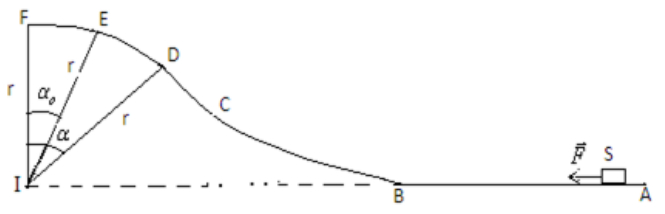
\includegraphics[width=0.5\textwidth]{./img/img00.jpg}
\end{center}

\begin{enumerate}
    \item  Donner l’énoncé du théorème de l’énergie cinétique \dotfill(0.5pt)
    \item  En appliquant le théorème de l’énergie cinétique sur le corps entre B et E , déterminer sa vitesse lors de son passage par le point B puis calculer sa valeur .\dotfill(1.5pts)
    \item En appliquant le théorème de l’énergie cinétique sur le corps entre A et B, déterminer l'intensité de la force $\vec{F}$ en fonction  de m , g et $\alpha_0$ puis calculer sa valeur.\dotfill(1.5pts)
    \item Sachant que pendant son retour du point E le corps S se déplace vers le point A . En appliquant le théorème de l’énergie cinétique sur le corps S entre D et E, déterminer l’expression de la vitesse $V_D$ du corps lors de son passage par le point D en fonction de g , r , $\alpha_0$ et $\alpha$ puis calculer sa valeur .\dotfill(1.5pts)
    \item Quelle vitesse qu’il fallait donner au corps au point B pour qu’il arrive au point F avec une vitesse nulle ? et dans ce cas qu'elle sera l'intensité de la force $\vec{F}$ ?\dotfill(1pt)


\end{enumerate}



%_________________partie 2  : gravitation universelle :)

\section*{Partie 2 : Travail mécanique d'une machine \dotfill (4pts)}
%\begin{wrapfigure}{r}{0.3\textwidth}
%\end{wrapfigure}

Une machine tournante a une fréquence de rotation égale à 200 tr/min. Son moment d'inertie par rapport à son axe de rotation est égal à $50 kg. m^2$ .

On prendra g = 10 N/ kg.
Pour l'arrêter on exerce une force tangentielle constante de 150 N.
\begin{enumerate}
    \item Calculer la variation d'énergie cinétique au cours du freinage.\dotfill(1pt)

\item Calculer le moment de la force de freinage sachant que la machine peut être assimilée à un disque de diamètre $80 cm$.\dotfill(1pt)

\item Calculer le nombre de tours effectués par la machine avant l'arrêt.\dotfill(2pts)
\end{enumerate}

\end{document}
